%% IMPORTANT: Once working, run latex 3 times to get listoffigures to work

%% Be sure to check spelling!

%% Put **your** name and the proper due date in place

%% Copy the lstlisting and figure code as many times as you need
%% Be sure to put in your own file names if appropriate

%% Note that the \epsfig commands are currently commented out - until the
%%%% files exist, processing this code without them will result in an error
%%%% so leave the comments until you have created the graphics files!

\documentclass{article}
\usepackage{amsmath}    % loads AMS-Math package
\usepackage{epsfig}     % allows PostScript files
\usepackage{listings}   % allows lstlisting environment
\usepackage{moreverb}   % allows listinginput environment
\usepackage[letterpaper, margin=0.75in]{geometry}  % set paper size/margins

\begin{document}
\begin{center}
\rule{6.5in}{0.5mm}\\~\\
\textbf{\large EGR 103L -- Fall 2017}\\~\\
\textbf{\huge Data Analysis}\\~\\
Ian Hanus (ih52)\\
Lab Section 1B, Wednesday 8:30-11:20 AM\\
24 September 2017\\~\\
{\small I understand and have adhered to all the tenets of the Duke
  Community Standard in completing every part of this assignment.  I
  understand that a violation of any part of the Standard on any part
  of this assignment can result in failure of this assignment, failure
  of this course, and/or suspension from Duke University.} 
\rule{6.5in}{0.5mm}\\
\end{center}
\tableofcontents
\listoffigures
\pagebreak

\section{Random Numbers}
Here is the diary created when the program runs:
\listinginput[1]{1}{RandDiary.txt}

\section{Hidden Images}
% discussion
The lab manual stated that the images could be found in the first, second, or third row and first, second, or third column. This created a 3x3 matrix where each point could be the starting point of the hidden image. The starting point of the hidden image scattered in every ninth row and sixteenth column of the original image could be changed simply by changing the starting position of an array search. For example, trying to find the hidden image starting in row two and column three in the coded array would look like CodedArray(2:9:end,3:16:end). Four images were found aside from the original array. Their starting coordinates in the matrix were (1,1),(1,2),(2,3), and (3,1).

\section{Chapra 2.18-2.19}
In the two graphs, every data point that was below the function line in figure 1 remained below the function line in figure 2. In figure 2 the function line is exponential whereas in figure one it is strictly linear. Also, the distribution along the x axis in figure 1 is evenly spaced whereas this is not the case for figure 2.

\section{Chapra 2.22}
% discussion - use \cite[p.~51]{Chapra}
The equations being plotted are each of the dimensions of the conical helix  with respect to $t$.
The equations are \cite[p.~51]{Chapra}:
\begin{align*}
x &= t\mbox{ cos(6t)}\\
y &= t\mbox{ sin(6t)}\\
z &= t\\
\end{align*}

\section{Weather Data Analysis}
The specific information weather information calculated is:
\listinginput[1]{1}{WeatherDiary.txt}
The noontime irradiance seems to follow a the path of a negative parabola with quite a bit of variation. It is highest toward the middle of the year, in the summer, whereas it is lowest during the winter. The January hourly temperature varies with the hour of the day. It is coldest in the night but begins to warm up as the day goes on, then drops again when night hits. This causes the pattern we see in the graph with very little variance from the expected pattern. The temperature does increase with the days very slightly at each time as the weather begins to warm up toward the end of January.

\pagebreak
\appendix
\section{Codes}
% Put the name of your file in the subsection name 
% and the listinginput input
% Be sure to include the community standard in codes!

% Add \pagebreaks if they make sense

% Put the files in the same order as the problems; generally, 
% scripts will come first followed by any functions called
% by those scripts.

\subsection{GenRand.m}
\listinginput[1]{1}{GenRand.m}
\clearpage
\subsection{FindMessages.m}
\listinginput[1]{1}{FindMessages.m}
\clearpage
\subsection{RunChapra02p18.m}
\listinginput[1]{1}{RunChapra02p18.m}
\clearpage
\subsection{RunCone.m}
\listinginput[1]{1}{RunCone.m}
\clearpage
\subsection{RunWeather.m}
\listinginput[1]{1}{RunWeather.m}

\clearpage % start Figures on new page

\section{Figures}

\begin{figure}[ht!]
\begin{center}
\epsfig{file=UniformPlot.eps, width=4.5in}
\caption{Histogram of Uniformly Distributed Random Numbers.}
\end{center}
\end{figure}

\begin{figure}[ht!]
\begin{center}
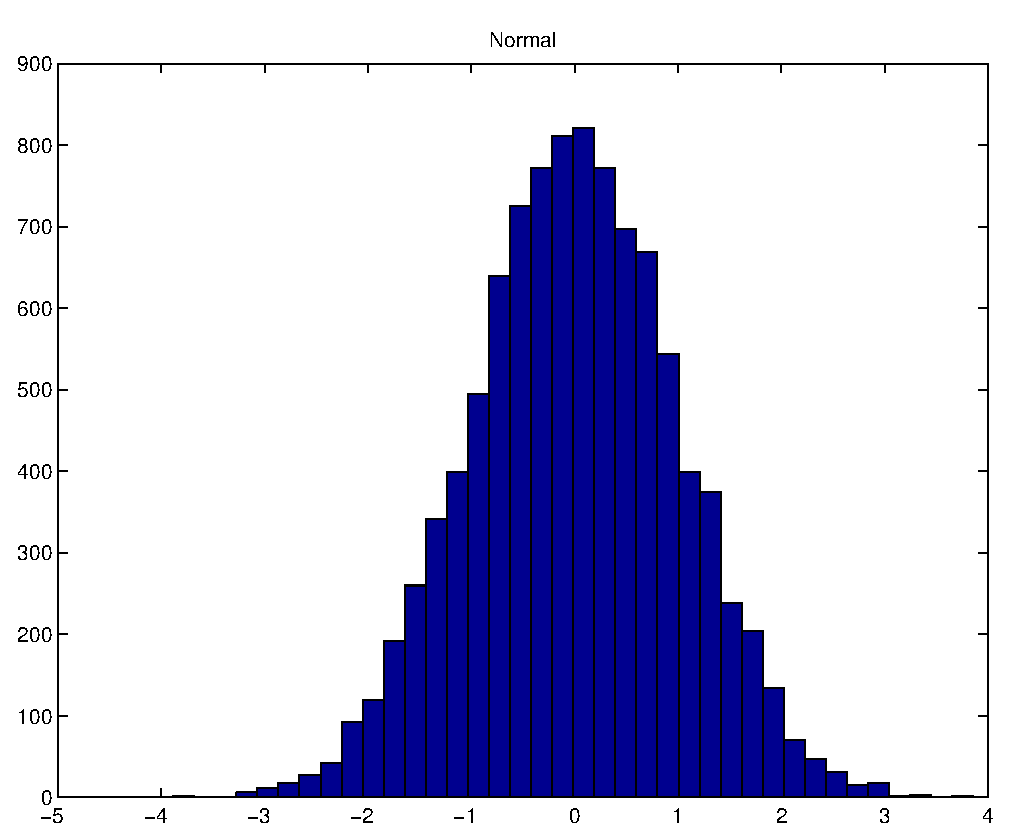
\epsfig{file=NormalPlot.eps, width=4.5in}
\caption{Histogram of Normally Distributed Random Numbers.}
\end{center}
\end{figure}

\begin{figure}[ht!]
\begin{center}
\epsfig{file=OriginalPlot.eps, width=4.5in}
\caption{Original Array.}
\end{center}
\end{figure}

\begin{figure}[ht!]
\begin{center}
\epsfig{file=GoodStartPlot.eps, width=4.5in}
\caption{First Image: ``Good Start.''}
\end{center}
\end{figure}

\begin{figure}[ht!]
\begin{center}
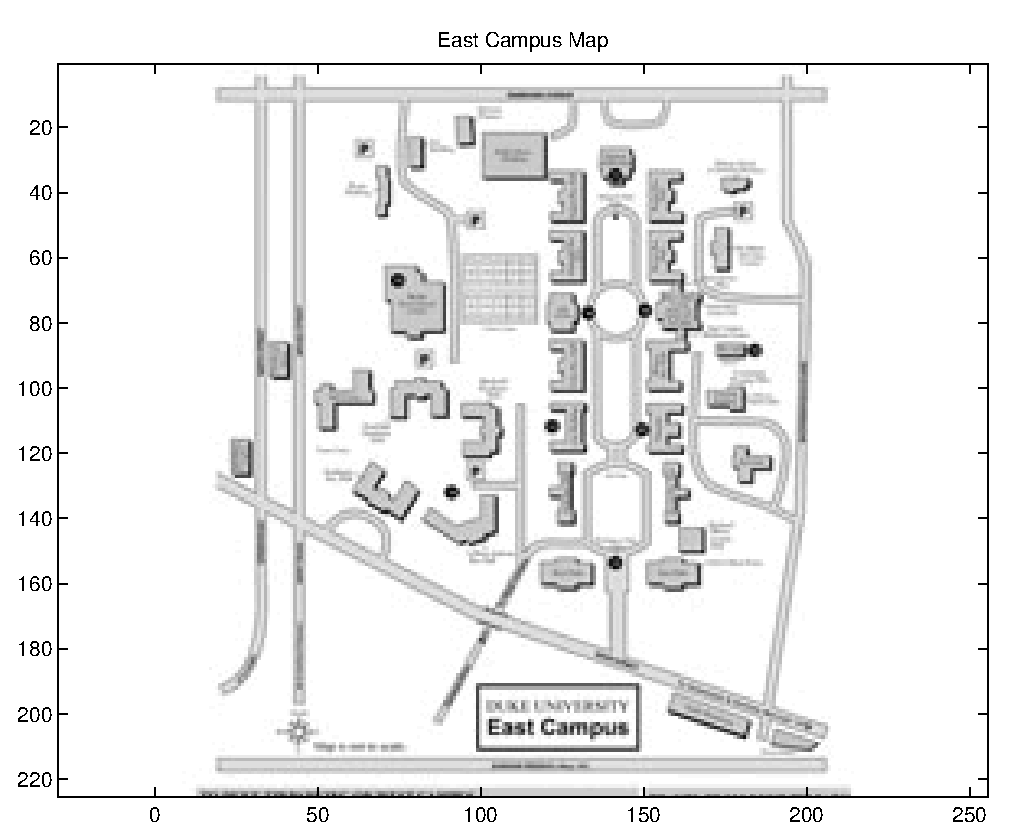
\epsfig{file=EastCampus.eps, width=4.5in}
\caption{Second Image: ``East Campus Map''}
\end{center}
\end{figure}

\begin{figure}[ht!]
\begin{center}

\epsfig{file=Pratt.eps, width=4.5in}
\caption{Third Image: ``Pratt School of Engineering''}
\end{center}
\end{figure}

\begin{figure}[ht!]
\begin{center}

\epsfig{file=Trinity.eps, width=4.5in}
\caption{Fourth Image: ``Trinity College of Arts \& Sciences''}
\end{center}
\end{figure}

% Repeat the above for the rest of the images.
\clearpage

\begin{figure}[ht!]
\begin{center}
\epsfig{file=WindPlotReg.eps, width=4.5in}
\caption{Wind Tunnel Forces: Regular Plot}
\end{center}
\end{figure}

\begin{figure}[ht!]
\begin{center}
\epsfig{file=WindPlotLog.eps, width=4.5in}
\caption{Wind Tunnel Forces: Log-Log Plot}
\end{center}
\end{figure}

\begin{figure}[ht!]
\begin{center}
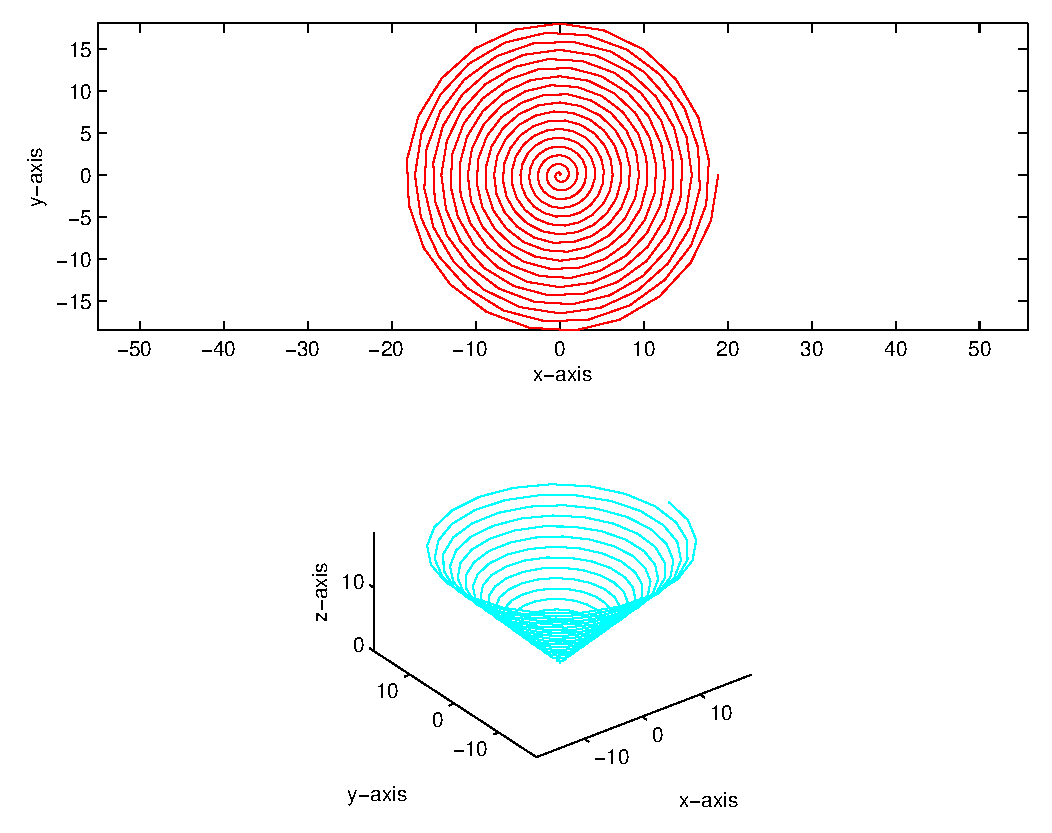
\epsfig{file=ConePlot.eps, width=4.5in}
\caption{Conical Helix Plots}
\end{center}
\end{figure}
\clearpage

\begin{figure}[ht!]
\begin{center}
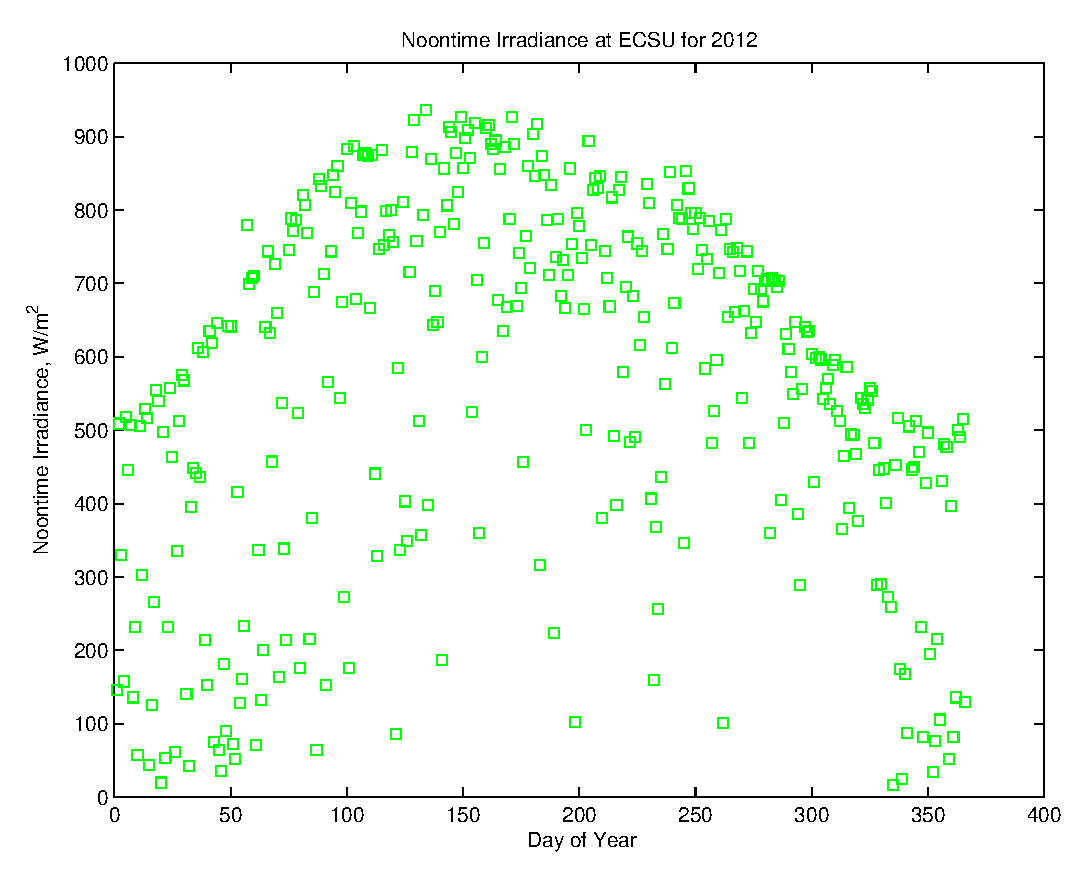
\epsfig{file=ORNLirrad.eps, width=4.5in}
\caption{Noontime Irradiance Plot}
\end{center}
\end{figure}

\begin{figure}[ht!]
\begin{center}
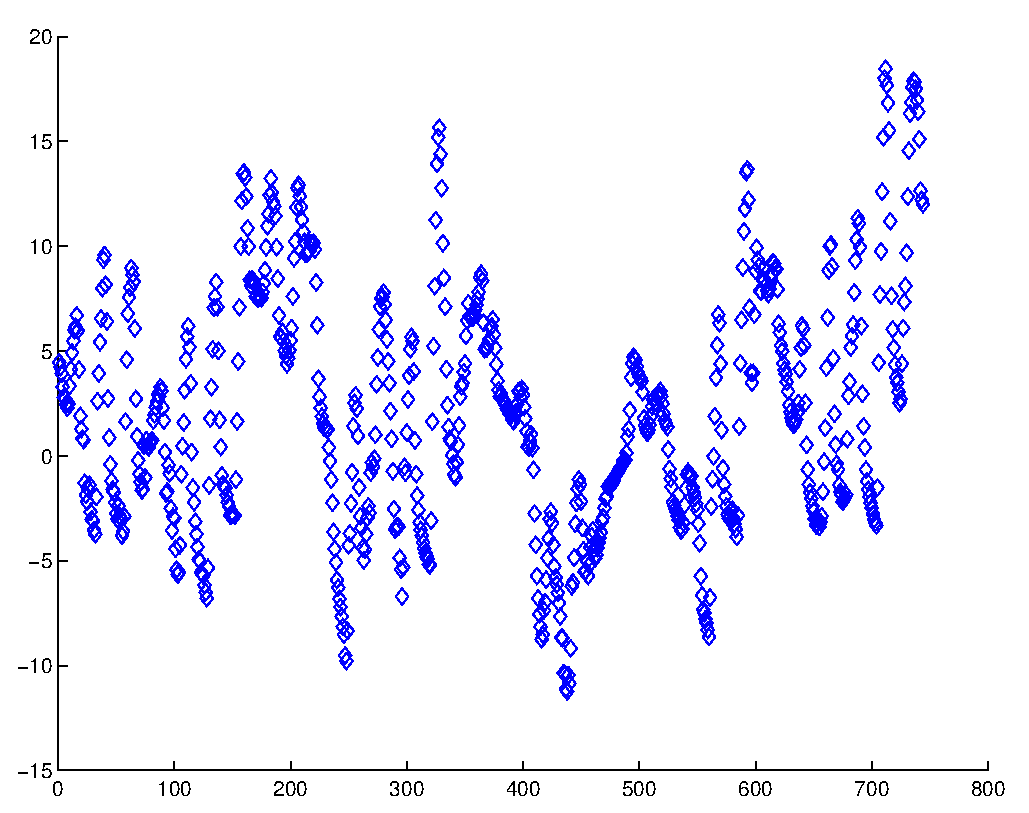
\epsfig{file=ORNLtemps.eps, width=4.5in}
\caption{January Temperatures Plot}
\end{center}
\end{figure}
\clearpage

\begin{thebibliography}{9}
\bibitem{Chapra}
  Chapra, Steven C.,
  {\it Applied Numerical Methods with MATLAB for Engineering and Scientists}.
  McGraw-Hill, New York,
  4th Edition,
  2018.
\end{thebibliography}

\end{document}

% LocalWords:  EGR 103L RandDiary txt Chapra WeatherDiary GenRand FindMessages
% LocalWords:  RunChapra02p18 RunCone RunWeather Irradiance MATLAB McGraw
